\chapter{Axissimetria}\label{parte_1}

\section{Procedimentos}
Para a implementação da simulação em questão foi seguido os seguintes procedimentos:
\begin{enumerate}
    \item Foram implementadas as condições anecóicas ao longo dos cantos do lattice, uma sobreposta a outra nos cantos;
    \item As barreiras foram implementadas nos cantos e no duto de forma separada entre eles;
    \item A condição de axissimetria foi implementada fazendo com que não haja reflxão não-física na parte aberta do lattice;
    \item O $chirp$ foi implementado utilizando a condição anecóica de massa variante e velocidade de partícula e mach 0.07 para os dois casos respectivamente.
\end{enumerate}

\section{Códigos}
Segue os códigos desenvolvidos:
\lstinputlisting{code/lista_3.m}
\lstinputlisting{code/build_anechoic_condition.m}
\lstinputlisting{code/build_source_anechoic.m}

\newpage
\section{Resultados}
Segue os gráficos obtidos:
\begin{figure}[h!]
    \centering
    \hspace{-1.5cm}
    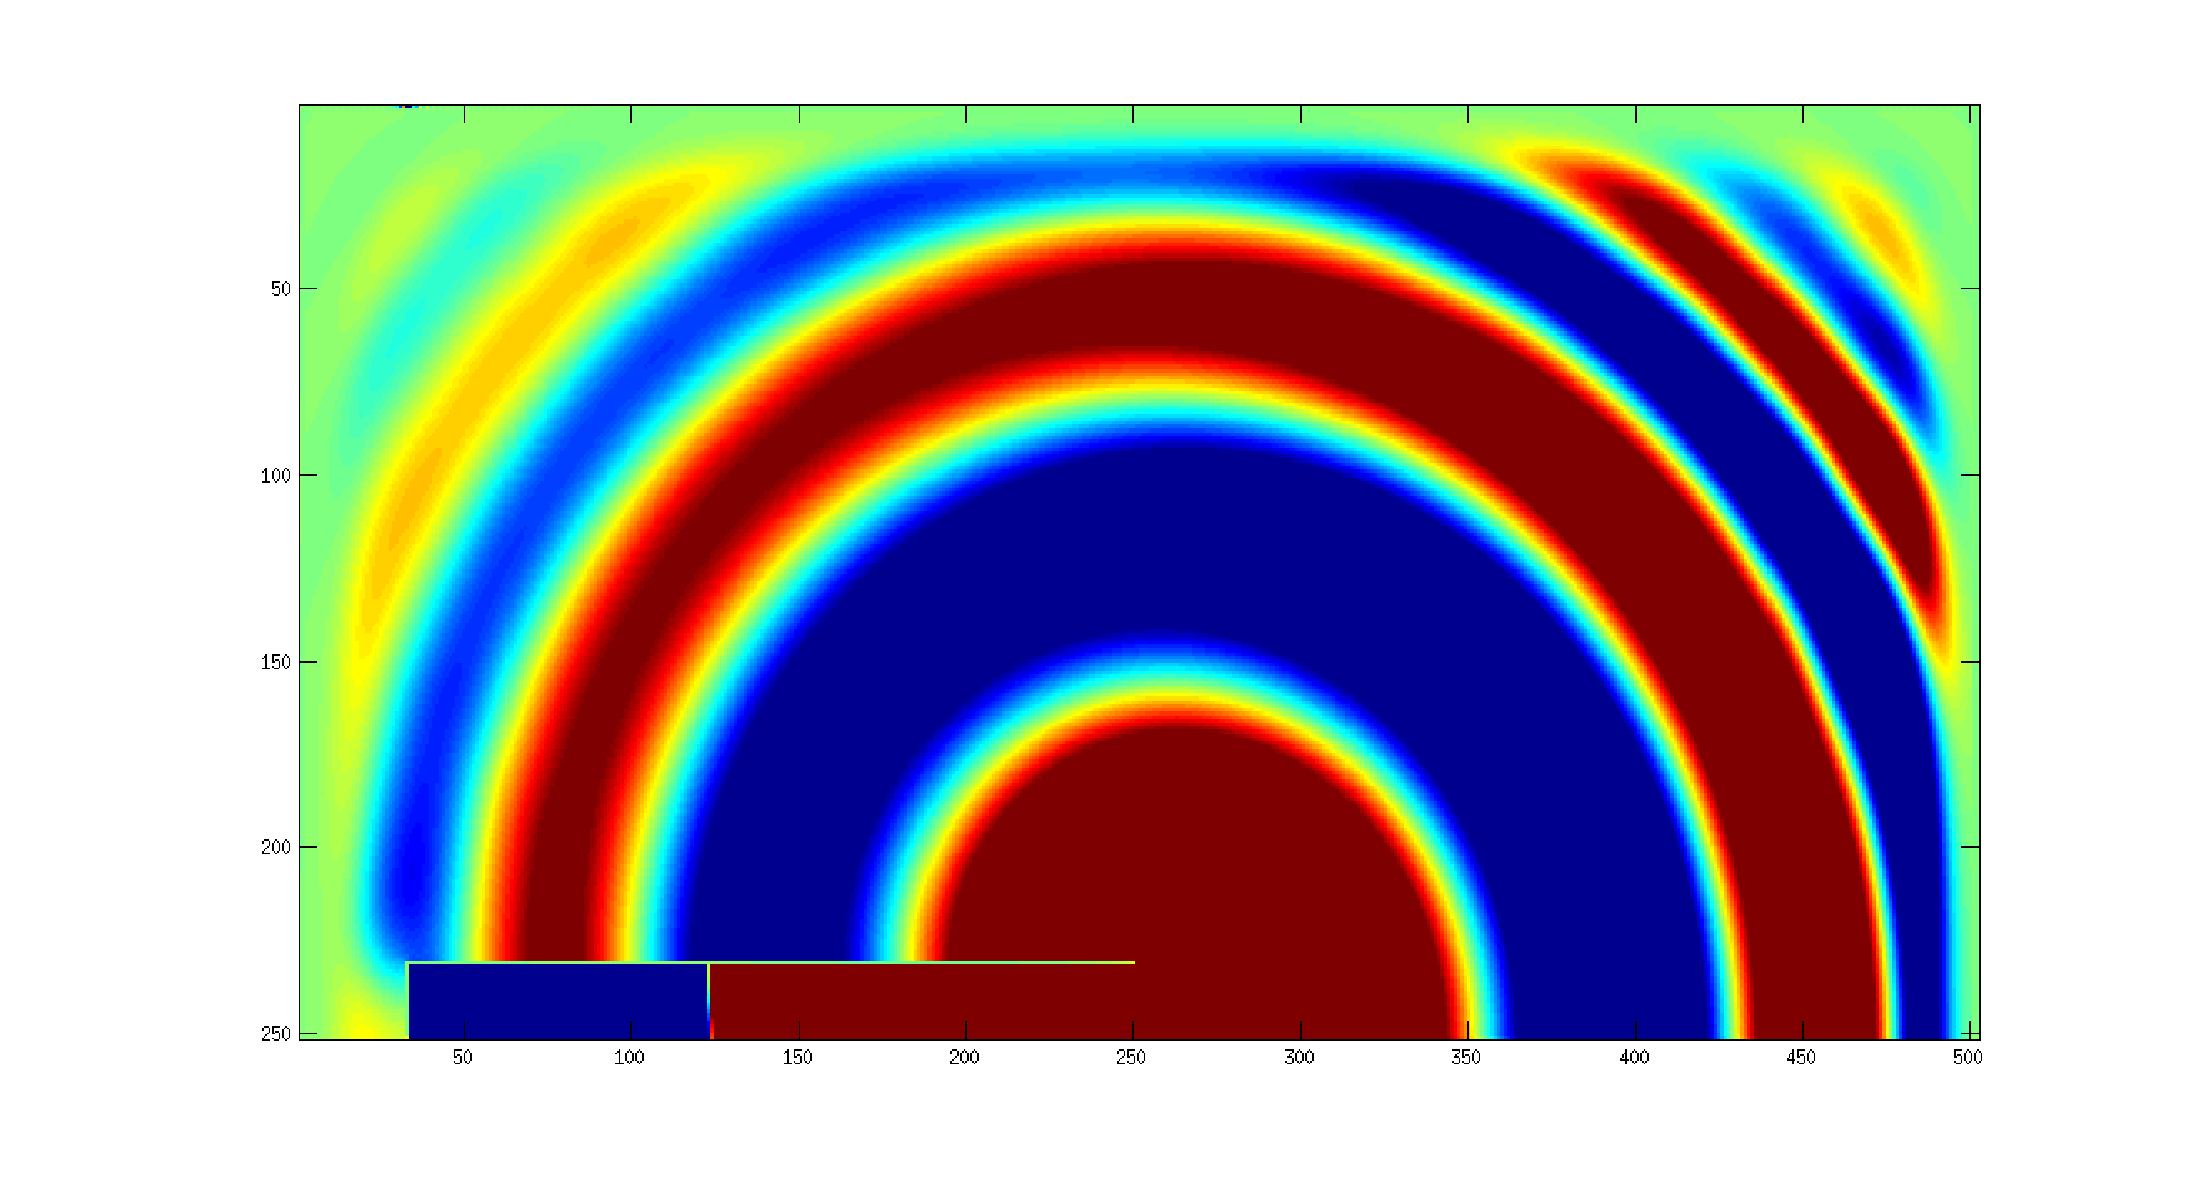
\includegraphics[width=0.8\textwidth]{code/simu.eps}
    \caption{Gráfico de densidades.}
\end{figure}
\begin{figure}[h!]
    \centering
    \hspace{-1.5cm}
    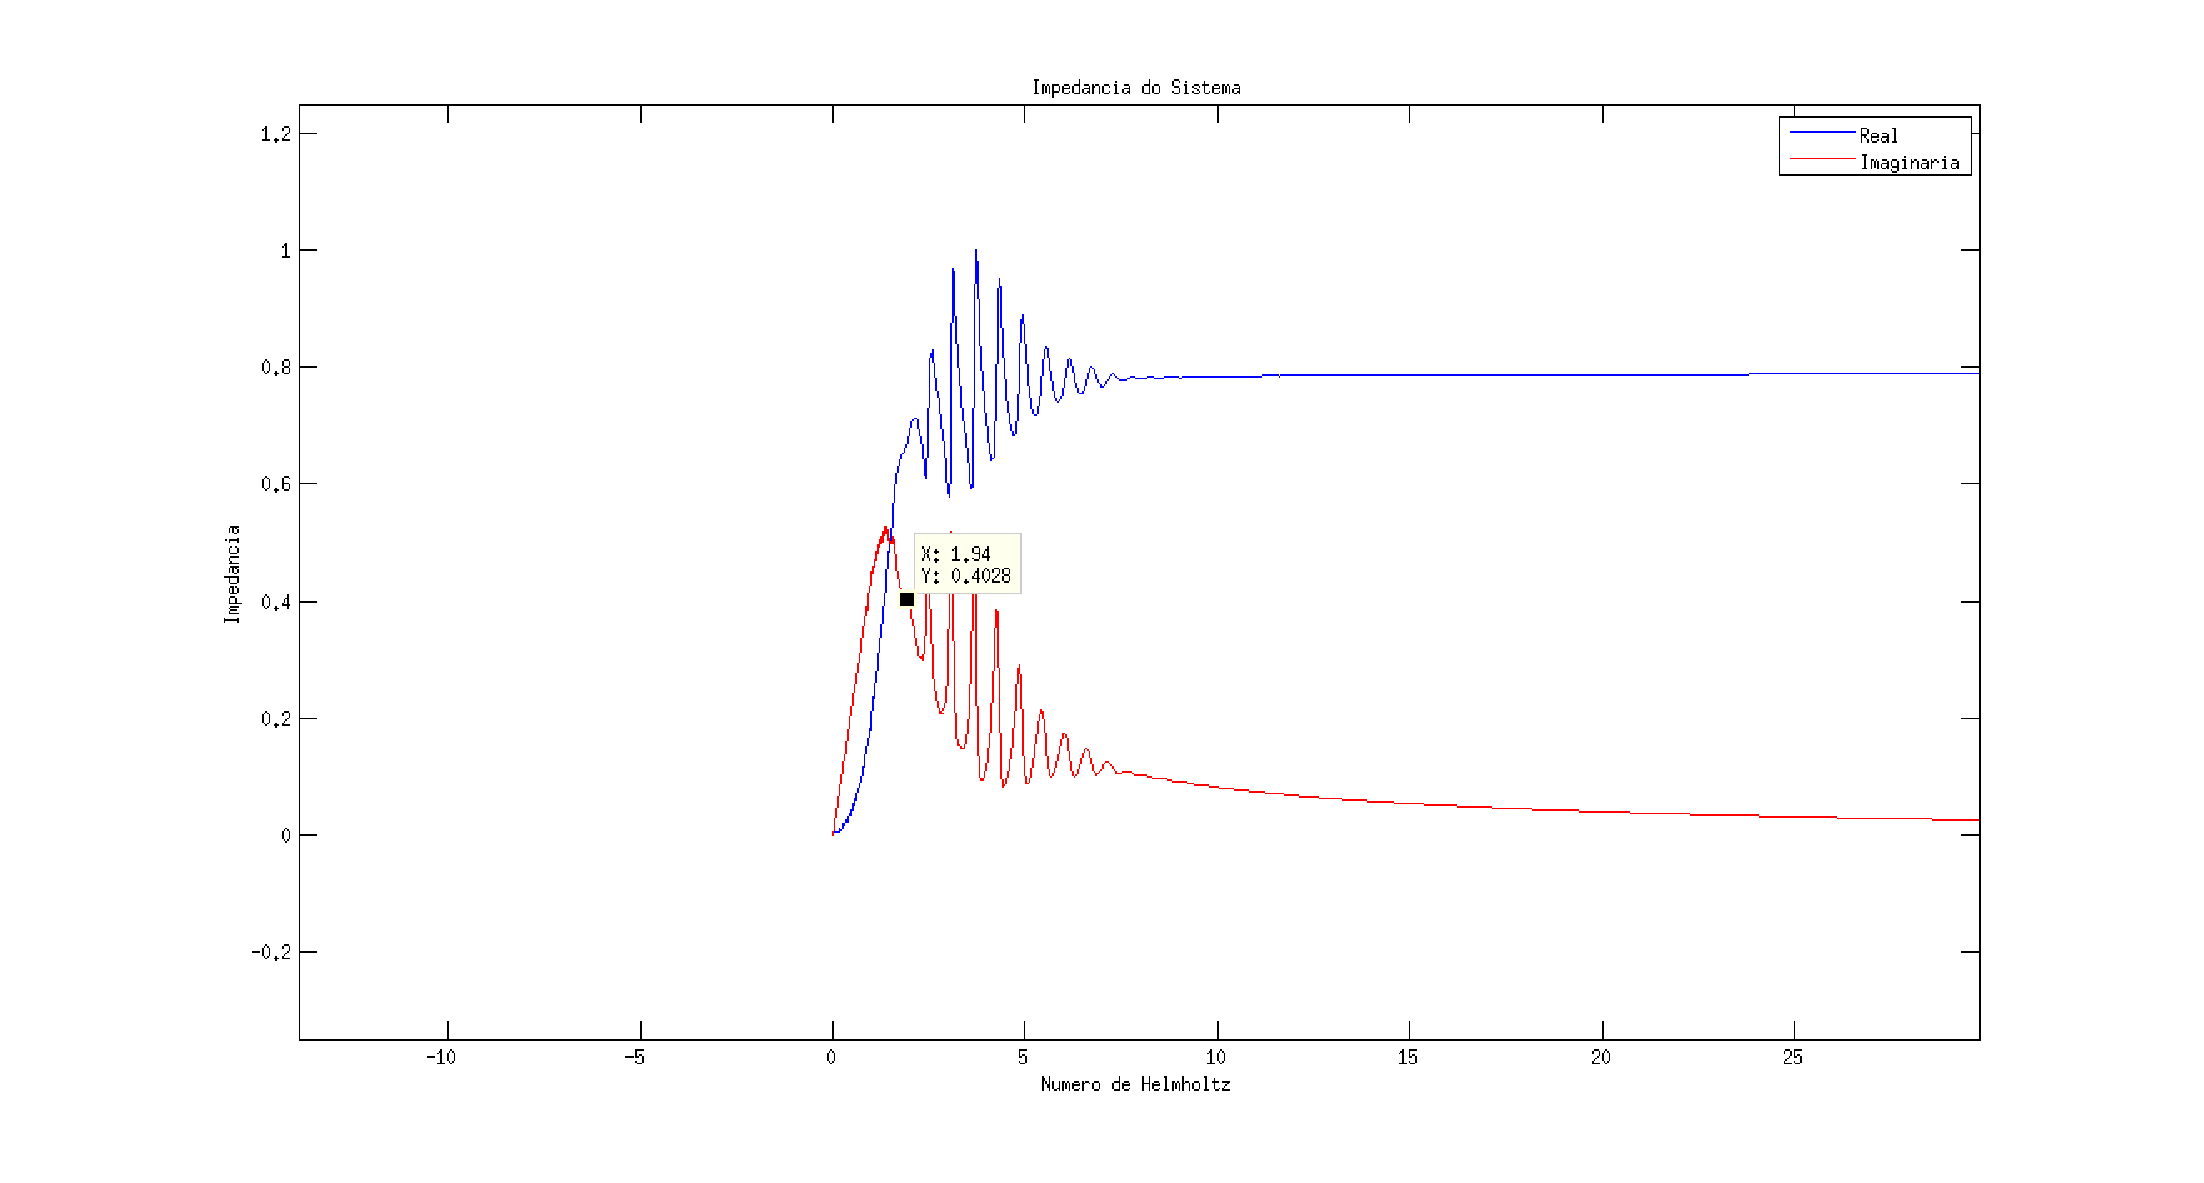
\includegraphics[width=1\textwidth]{code/impedancia_sem.eps}
    \caption{Gráfico de impedância sem escoamento.}
\end{figure}

\newpage
\begin{figure}[t!]
    \centering
    \hspace{-1.5cm}
    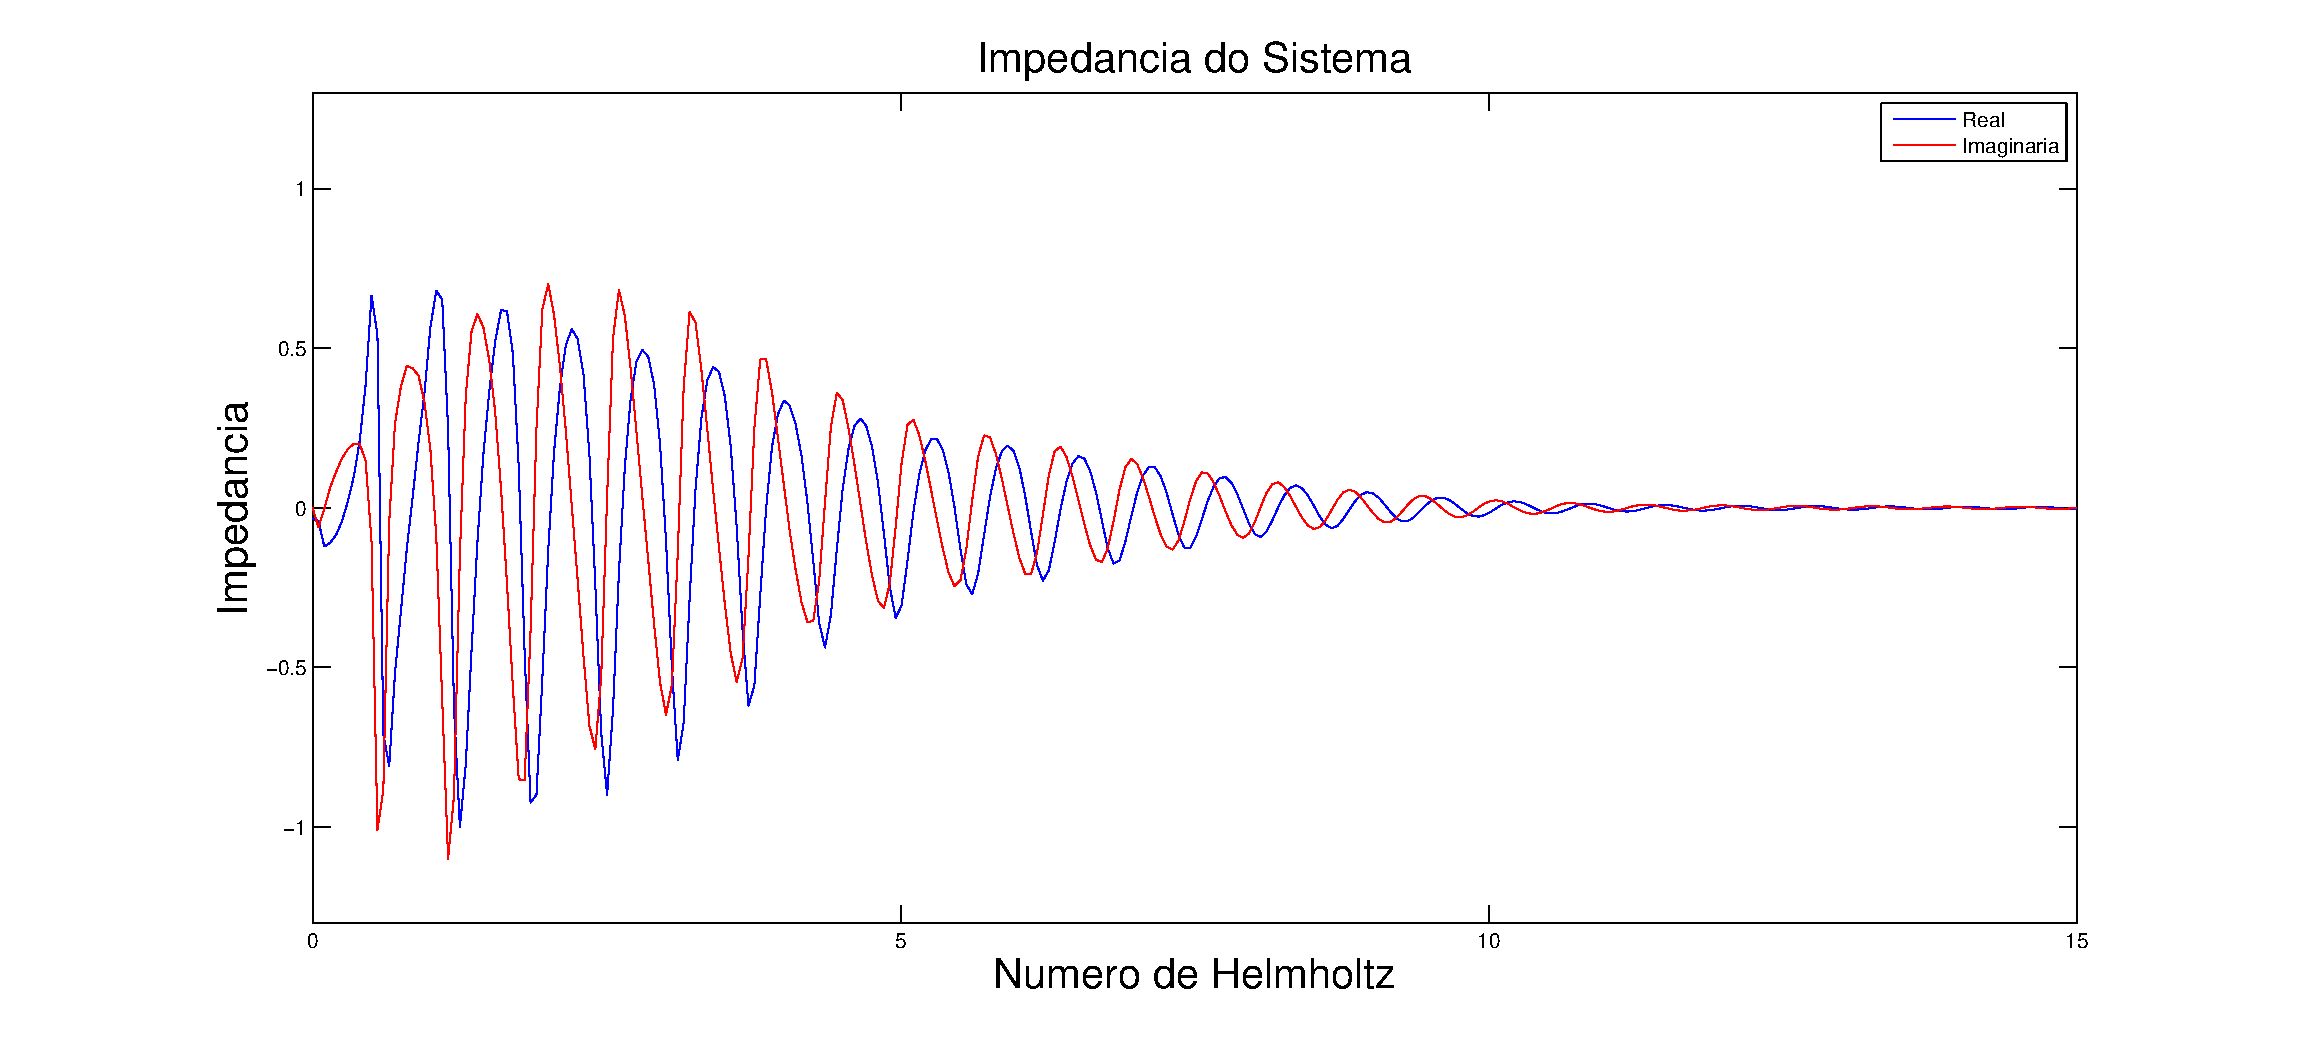
\includegraphics[width=1\textwidth]{code/impedancia_com.eps}
    \caption{Gráfico de impedância com escoamento (Mach = 0.07).}
\end{figure}


%\lstinputlisting{code_matlab/code_refactored/closed-closed/main_lbgk.m}

\chapter{Paredes Não-Alinhada}\label{parte_1}

Para o desenvolvimento dessa questão foi criada uma nova função com essa assinatura:
\begin{lstlisting}
    function [q, vecloc] = funcao(i, vecx, vecy, Nr, Mc)
\end{lstlisting}

Ela recebe os parâmetros de número de colunas (Nr), número de colunas (Mc), pontos da parede não-alinhada ao longo da ordenada (vecy), pontos da parede não-alinhada ao longo da abscissa (vecx) e direção da célula lattice (i) que pode variar de 1 a 9. Nesse caso só foi possível implementar na direção 1, ou seja, todas as células que cruzam para a direita a barreira não-alinhada. De retorno a função devolve a matriz das distâncias das células que cruzam a barreira (q) e a matriz de células que cruzam a barreira.

O algorítmo pensado para resolver esse problema possui os seguintes passos:
\begin{enumerate}
    \item Verificar se os pontos da barreira estão dentro do tamanho da matriz de lattice:
    \begin{lstlisting}
    % verify if the points is inside of lattice
    is_not_points_inside_lattice = ... 
    min(vecx) < 1 || max(vecx) > Mc ...
    || min(vecy) < 1 || max(vecy) > Nr;
    if is_not_points_inside_lattice
        i = -1;
        message = 'The points x and y are outside of lattice.';
        disp(message);
    end
    \end{lstlisting}
    \item Assumir uma rota de processamento para a direção lattice $i$ inserida:
    \begin{lstlisting}
    if i == 1
    \end{lstlisting}
    \item Restringir o domínio de lattice num quadrado de tamanho mínimo que caiba toda a barreira não-alinhada:
    \begin{lstlisting}
    vecloc = zeros(Nr, Mc);
    q = zeros(Nr, Mc);
    % square that have the entire points
    square_x = [floor(min(vecx)) ceil(max(vecx))];
    square_y = [floor(min(vecy)) ceil(max(vecy))];
    \end{lstlisting}
    \item Ir iterando em todas as alturas dentro do quadrado mínimo calculado:
    \begin{lstlisting}
    for point_y = square_y(1):square_y(2)
    \end{lstlisting}
    \item Calcular os dois pontos mais próximos para fazer a interpolação:
    \begin{lstlisting}
    % looking for a x point 
    % (Verify whats p1 and p2 is nearest from height)
    distances_y = abs(vecy - point_y);
    slot_min = find(distances_y == min(distances_y));
    p2_y = vecy(slot_min);
    p2_x = vecx(slot_min);
    distances_y(slot_min) = 10e10;
    slot_min = find(distances_y == min(distances_y));
    p1_y = vecy(slot_min);
    p1_x = vecx(slot_min);
    \end{lstlisting}
    \item Realizar a interpolação linear:
    \begin{lstlisting}
    % Agora tenho p1 e p2, tenho que agora fazer a
    % interpolacao linear para achar o p3 
    % equacao da reta: y = ax + b
    a = (p2_y - p1_y)/(p2_x - p1_x);
    b = p1_y - a*p1_x;
    p3_x = (point_y - b)/a;
    \end{lstlisting}
    \item Calculando a distância e adquirindo a célula que cruza a barreira a direita:
    \begin{lstlisting}
    % e calcular a distancia em x do ponto que eu to para o x de p3
    distances_points = [square_x(1):square_x(2)] - p3_x;
    distances_points = abs(distances_points);
    point_x = find(distances_points == min(distances_points));
    vecloc(point_y, point_x) = 1;
    q(point_y, point_x) = min(distances_points);
    \end{lstlisting}
\end{enumerate}

Segue o código em sua totalidade:
\lstinputlisting{code/funcao.m}

Também segue o script para o teste da função criada:
\lstinputlisting{code/teste_funcao.m}

Para o cálculo do quadrado mínimo que abrange a barreira não-alinhada foi adiquirido tais resultados:
\begin{figure}[h!]
    \centering
    \hspace{-1.5cm}
    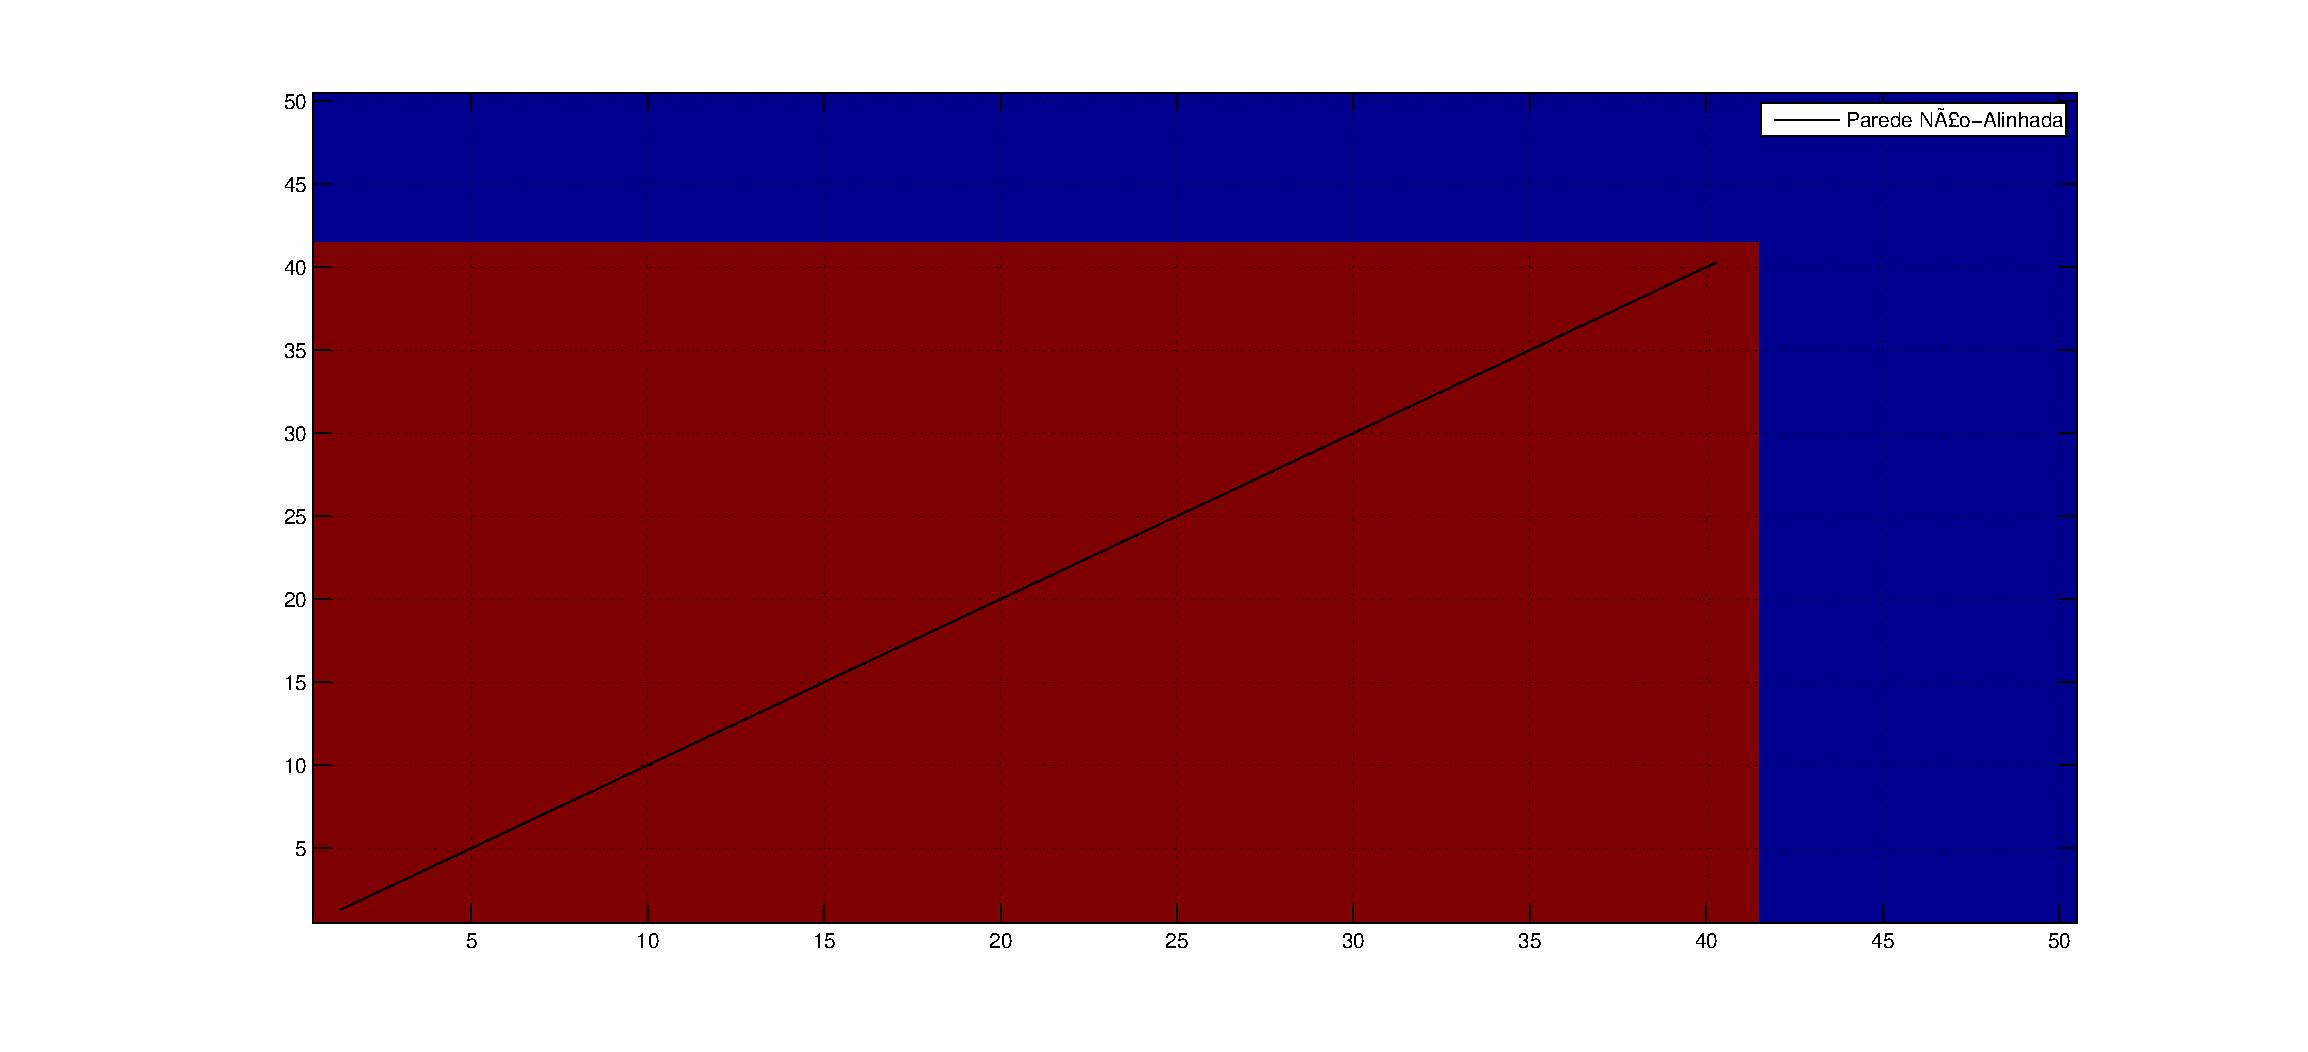
\includegraphics[width=0.8\textwidth]{code/quadrado_1.eps}
    \caption{Barreira não-alinhada reta e deslocada em 0.3.}
\end{figure}
\begin{figure}[h!]
    \centering
    \hspace{-1.5cm}
    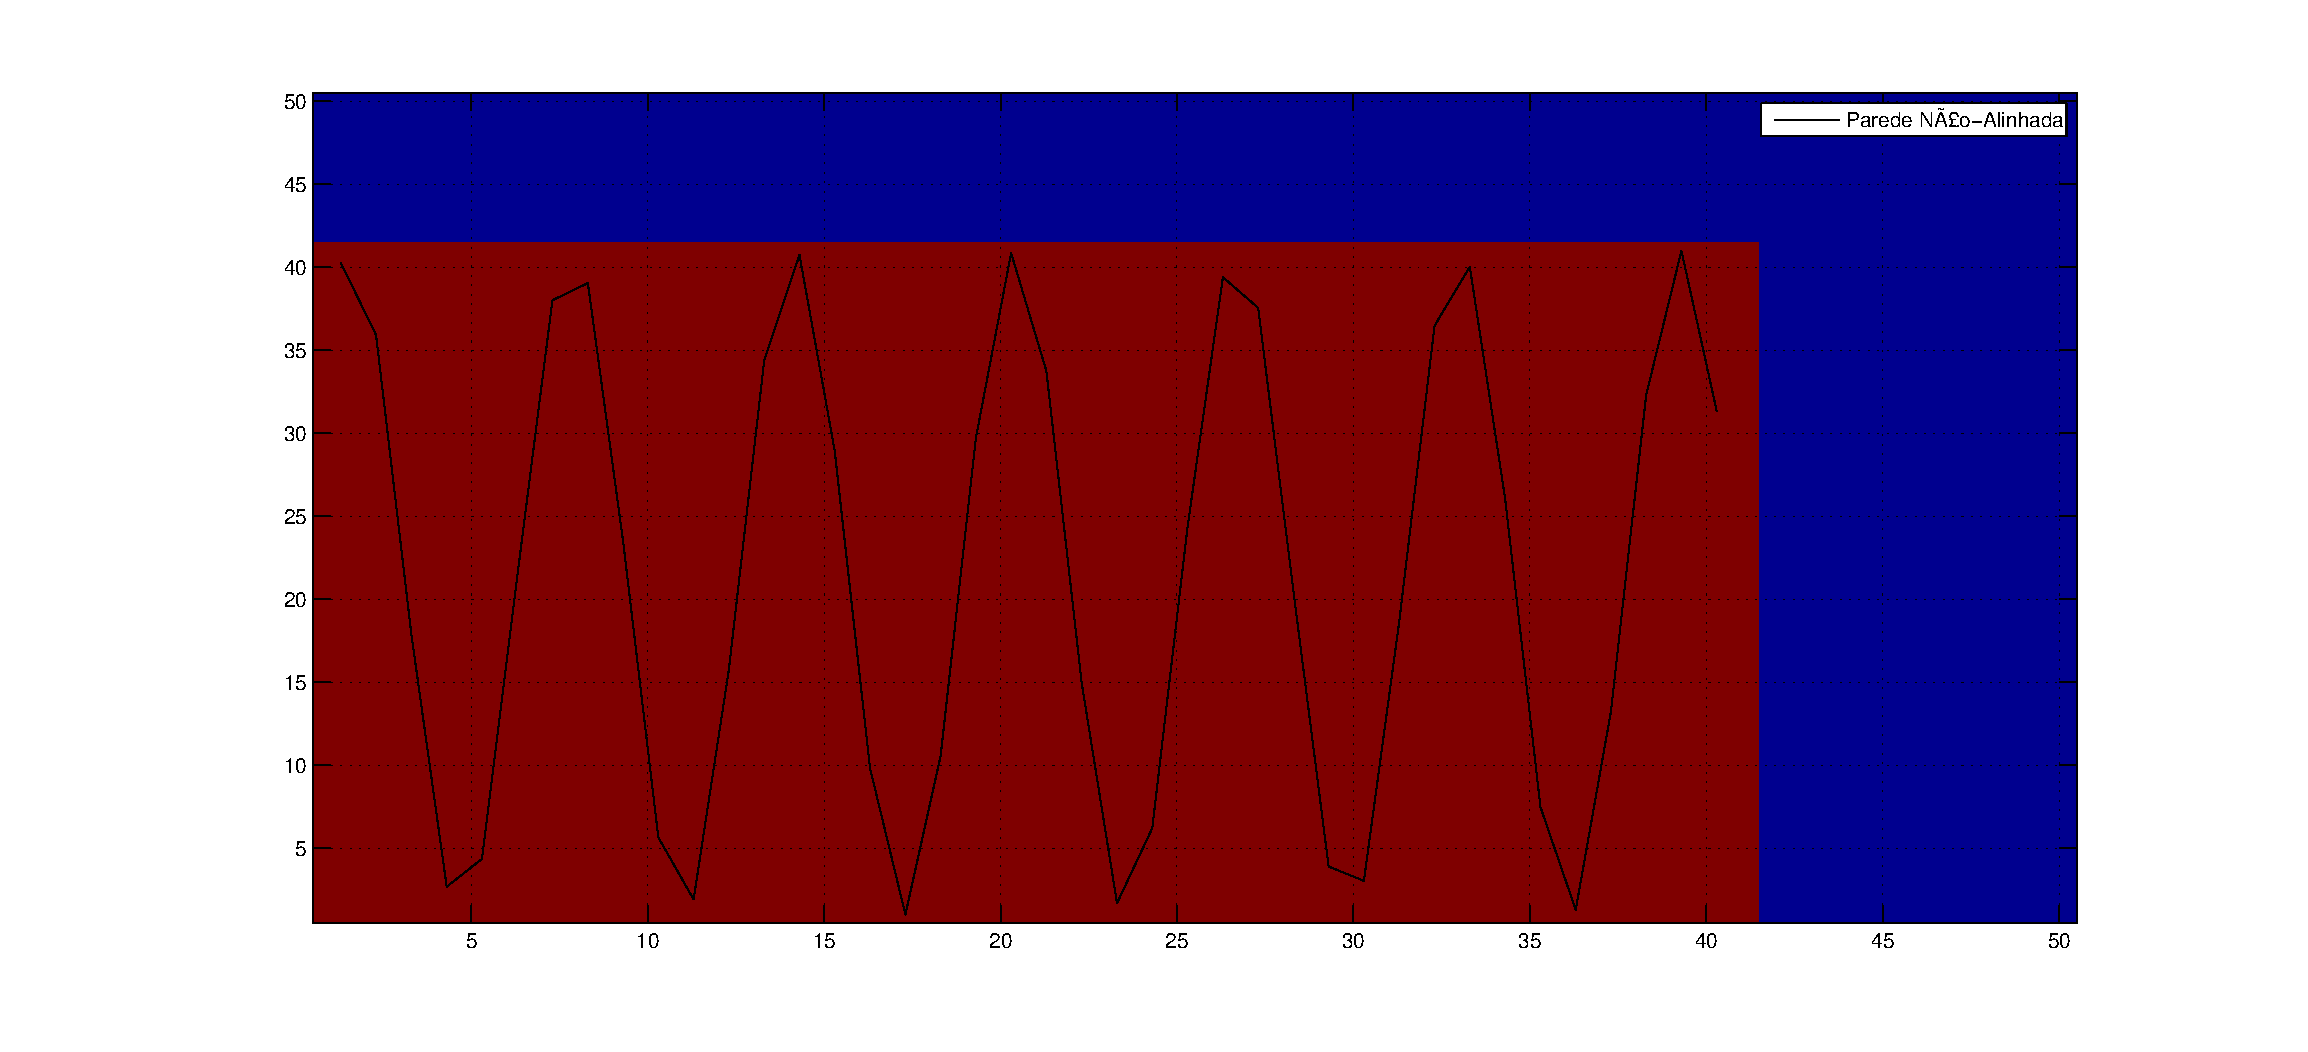
\includegraphics[width=0.8\textwidth]{code/quadrado_2.eps}
    \caption{Barreira não-alinhada senoidal.}
\end{figure}

Para o cálculo das células que atravessam a barreira pela direita segue os resultados:
\begin{figure}[h!]
    \centering
    \hspace{-1.5cm}
    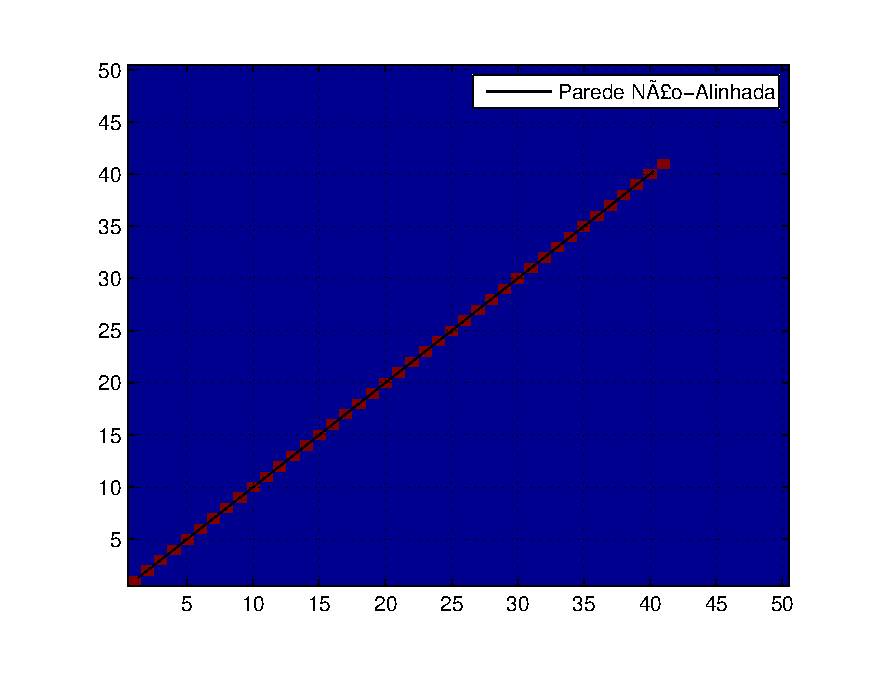
\includegraphics[width=0.8\textwidth]{code/cruza_1.eps}
    \caption{Células de Lattice que cruzam barreira não-alinhada reta e deslocada em 0.3.}
\end{figure}
\begin{figure}[h!]
    \centering
    \hspace{-1.5cm}
    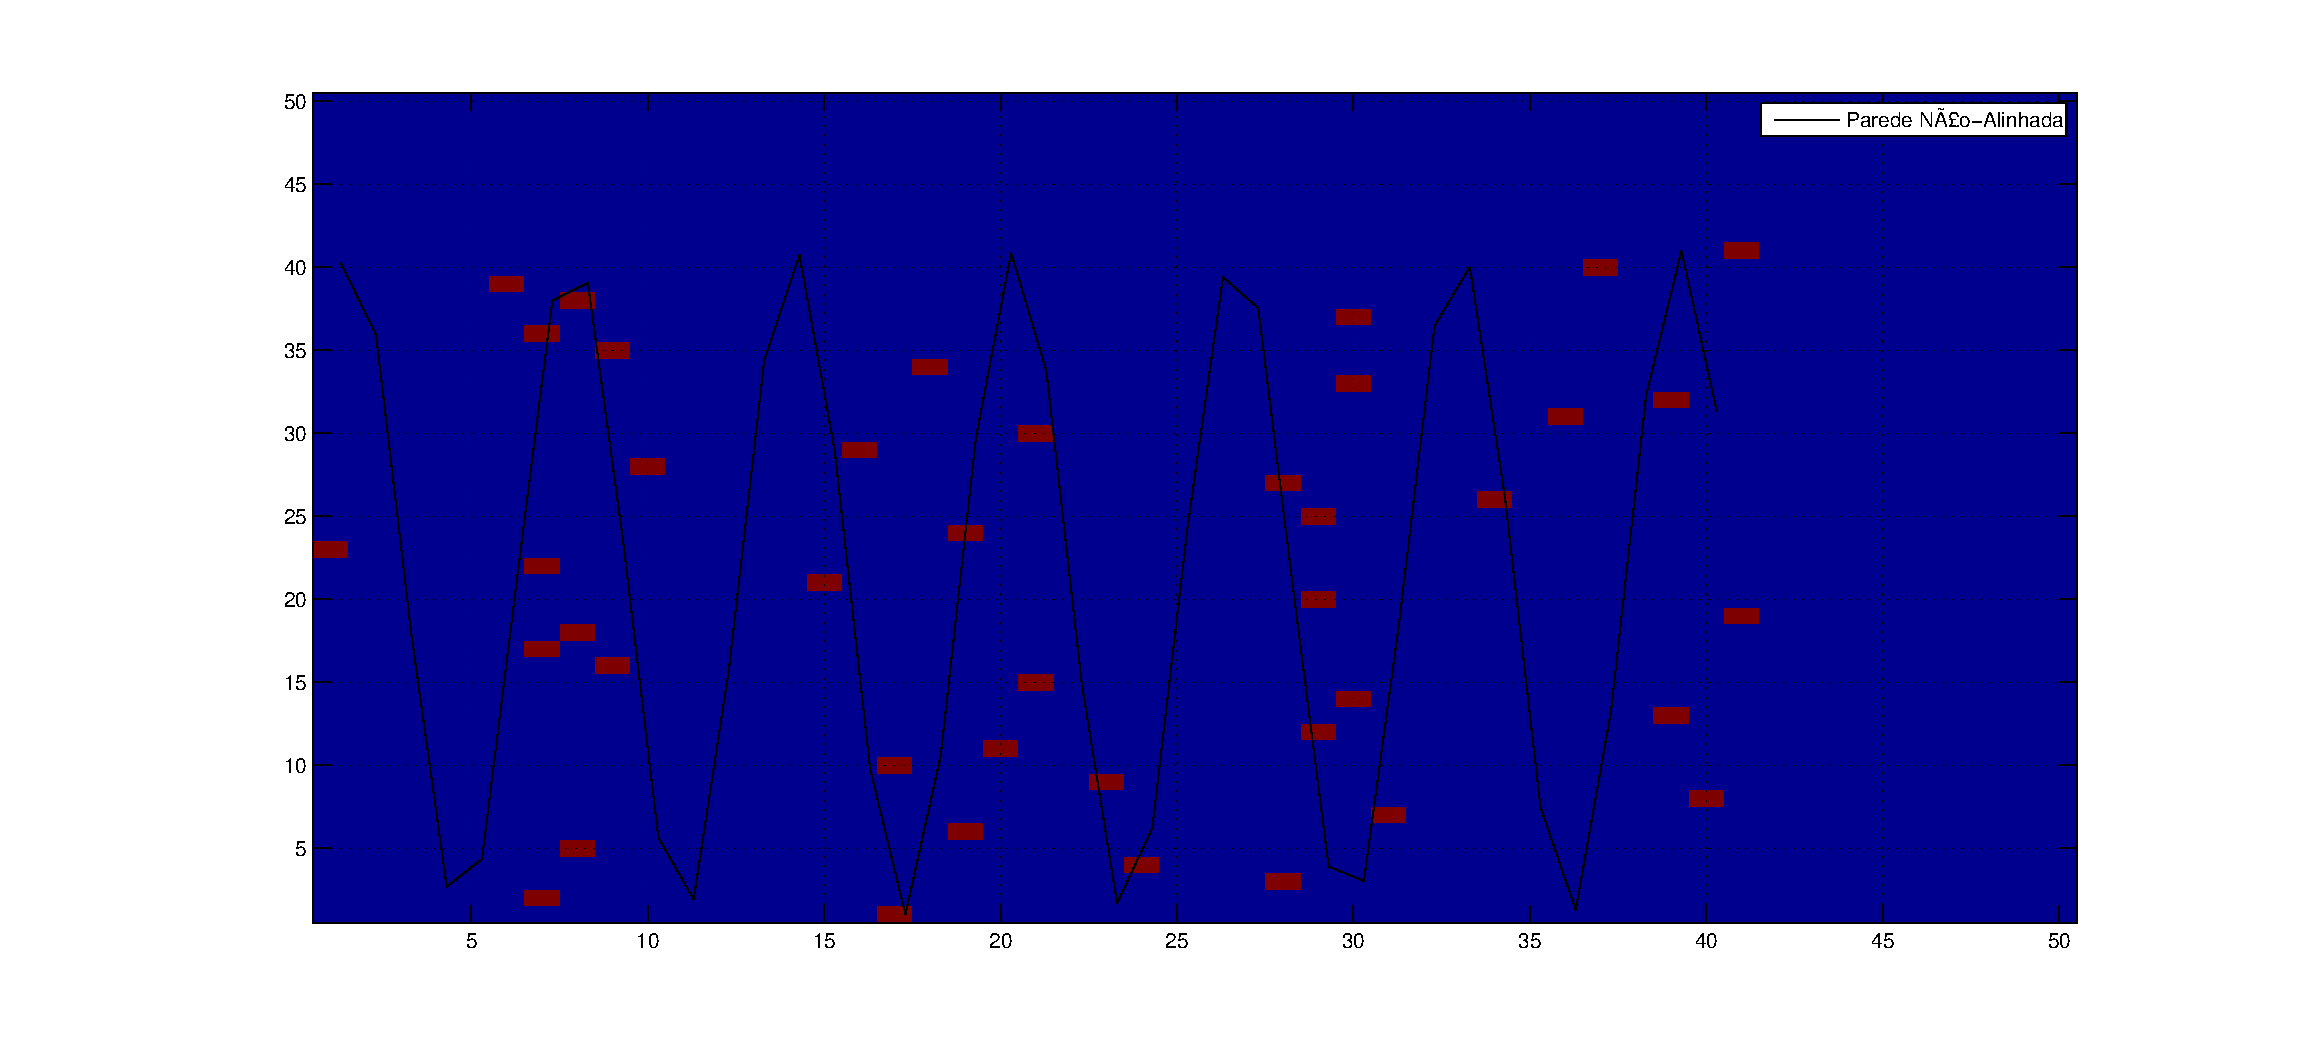
\includegraphics[width=0.8\textwidth]{code/cruza_2.eps}
    \caption{Células de Lattice que cruzam em barreira não-alinhada senoidal.}
\end{figure}
